% !TeX document-id = {a24bb292-b05f-4465-9a19-f6adbf8b8362}
%% A simple template for a term report using the Hagenberg setup
%% based on the standard LaTeX 'report' class
%%% äöüÄÖÜß  <-- no German umlauts here? Use an UTF-8 compatible editor!

%%% Magic comments for setting the correct parameters in compatible IDEs
% !TeX encoding = utf8
% !TeX program = pdflatex 
% !TeX spellcheck = en_US
% !BIB program = biber

\RequirePackage[utf8]{inputenc} % Remove when using lualatex or xelatex!
\RequirePackage{hgbpdfa}        % Creates a PDF/A-2b compliant document

\documentclass[english,notitlepage,smartquotes]{hgbreport}
% Valid options in [..]: 
%    Main language: 'german' (default), 'english'
%    Turn on smart quote handling: 'smartquotes'
%    APA bibliography style: 'apa'
%    Do not create a separate title page: 'notitlepage'
%%%-----------------------------------------------------------------------------

\graphicspath{{images/}}  % Location of images and graphics
\bibliography{references} % Biblatex bibliography file (references.bib)

%%%-----------------------------------------------------------------------------
\begin{document}
%%%-----------------------------------------------------------------------------

\author{Tobias Kothbauer, Veronika Leitner}                    % Your name
\title{Guide Guru - Interactive Travel Guide Project Report}	                 % or "Project Report"
\date{\today}

%%%-----------------------------------------------------------------------------
\maketitle
%%%-----------------------------------------------------------------------------

\begin{abstract}\noindent
In today's ever-changing world of travel, Guide Guru steps forward as a personal solution, ready to revolutionize how users embark on their journeys. Rooted in the fusion of cutting-edge technology and user-centric design philosophy, this project endeavors to craft a travel guide application that avoids limitations of traditional planning methods. 

\bigskip
\noindent At its core, Guide Guru is driven by the vision of empowering travelers with a personalized experience, one that seamlessly aligns with their interests, preferences and hobbies. Leveraging the capabilities of advanced large language models, the application will function as an intuitive digital companion, which adapts to the desires of each user. By fostering a tight relationship between technology and user input, Guide Guru endeavors to simplify the travel planning process, offering a platform where every journey is curated to reflect the personality of the individual. 

\bigskip
\noindent
\end{abstract}

%%%-----------------------------------------------------------------------------
\tableofcontents
%%%-----------------------------------------------------------------------------

%%%-----------------------------------------------------------------------------
\chapter{Aims and Context}
%%%-----------------------------------------------------------------------------

The core objective of this project is to develop an intuitive and adaptable travel guide application that seamlessly integrates user input with language processing capabilities. Through the implementation of user surveys, Guide Guru should gather and evaluate individual interests, ensuring that every travel recommendation is finely tuned to match the user's specific desires and hobbies.

The envisioned application gives users a tool with a simple interface, allowing them to effortlessly select destinations and specify personal interests, thereby generating travel guides curated to their liking.

Moreover, Guide Guru will offer the practical functionality of exporting personalized guides in PDF format, enabling users to conveniently access their curated recommendations on various devices and platforms.

Upon completion, Guide Guru targets delivering a travel companion, that eases the planning process and allows a high levels of customization and efficiency. By placing the user at the center of the experience, Guide Guru aims to enhance the quality of travel adventures, empowering individuals to craft marvelous journeys that align, with their interests and preferences.

In order to accurately reflect user preferences in Guide Guru, a questionnaire was created. Thirty-three participants provided insights into their travel habits, hobbies, interests, and their perspectives on the ideal format for a travel guide. This data has allowed us to customize Guide Guru to cater to a diverse audience, requiring minimal user input while still meeting their needs effectively.

%%%-----------------------------------------------------------------------------
\chapter{Project Details}
%%%-----------------------------------------------------------------------------
%Describe important project steps, \eg, the rationale of the chosen architecture
%or technology stack, design decisions, algorithms used, interesting challenges
%faced on the way, lessons learned \etc
Throughout our project, we carefully navigated through crucial steps to ensure success and produce great outcomes for our Guide Guru. From crafting detailed surveys to choosing the best technology tools, our path was defined by strategic choices aimed at crafting a tailored and efficient travel guide experience.

\section{Questionaire}

Initially, we developed a questionnaire based on our understanding of the essential information required to create a straightforward yet impactful prototype with highly personalized outcomes.

This survey included questions about user preferences, assessments of the importance of different travel factors, and open-ended questions to uncover insights into hobbies and preferred content for the travel guide.

Key findings from the survey revealed that the majority of participants preferred selecting their destination rather than receiving recommendations. Primary considerations for their travels included the type of travel (\eg, relaxation vacation), the overall environment (\eg, beach or city), and the preferred season for travel. Discovering new hobbies ranked as the least important aspect. All participants expressed a preference for receiving the travel guide in PDF format, with a strong emphasis on the importance of suitable images. Additionally, 85\% favored selecting their hobbies from a predefined list, with sports and art \& culture emerging as the most frequently mentioned categories. Regarding desired information in the travel guide, participants highlighted sights and hidden gems, culinary recommendations, entertainment options, cultural insights, and information on country-specific risks and hazards.

\section{Technology Stack}
Simultaneously, we conducted research on potential technology stacks. Two components were predetermined: utilizing React\footnote{https://react.dev} for frontend development to enhance our web development skills with this technology, and selecting ChatGPT from OpenAI\footnote{https://openai.com} as our preferred large language model (LLM), thus our supervisor thankfully could provide us with an API key for this model.

Following several iterations, we opted to employ Python\footnote{https://www.python.org} for backend development after discovering its well-documented approach to integrating a LLM into a web application. As well Flask\footnote{https://flask.palletsprojects.com/en/3.0.x/}, a micro web framework, was chosen to handle requests and CORS policies.

Given the importance of images as indicated by survey participants, and considering the multitude of cities and places of interest generated by user input, we needed a means to access online data for countless locations. To achieve this, we utilized a combination of the Google Places API\footnote{https://developers.google.com/maps/documentation/places/web-service/overview?hl=de} and Google Photos API\footnote{https://developers.google.com/photos?hl=de} to download and display images from user recommendations, providing users with a simple yet effective insight into selected destinations.

To validate user input for potential travel destinations, we integrated the geonames API\footnote{https://www.geonames.org}, which is user-curated and lists millions of places, allowing filtering for highly populated areas. This API facilitated the inclusion of destinations with populations exceeding 1000, ensuring a diverse range of travel destinations could be used to generate the guide.

\section{Prototype Design}

\begin{figure}
	\centering
	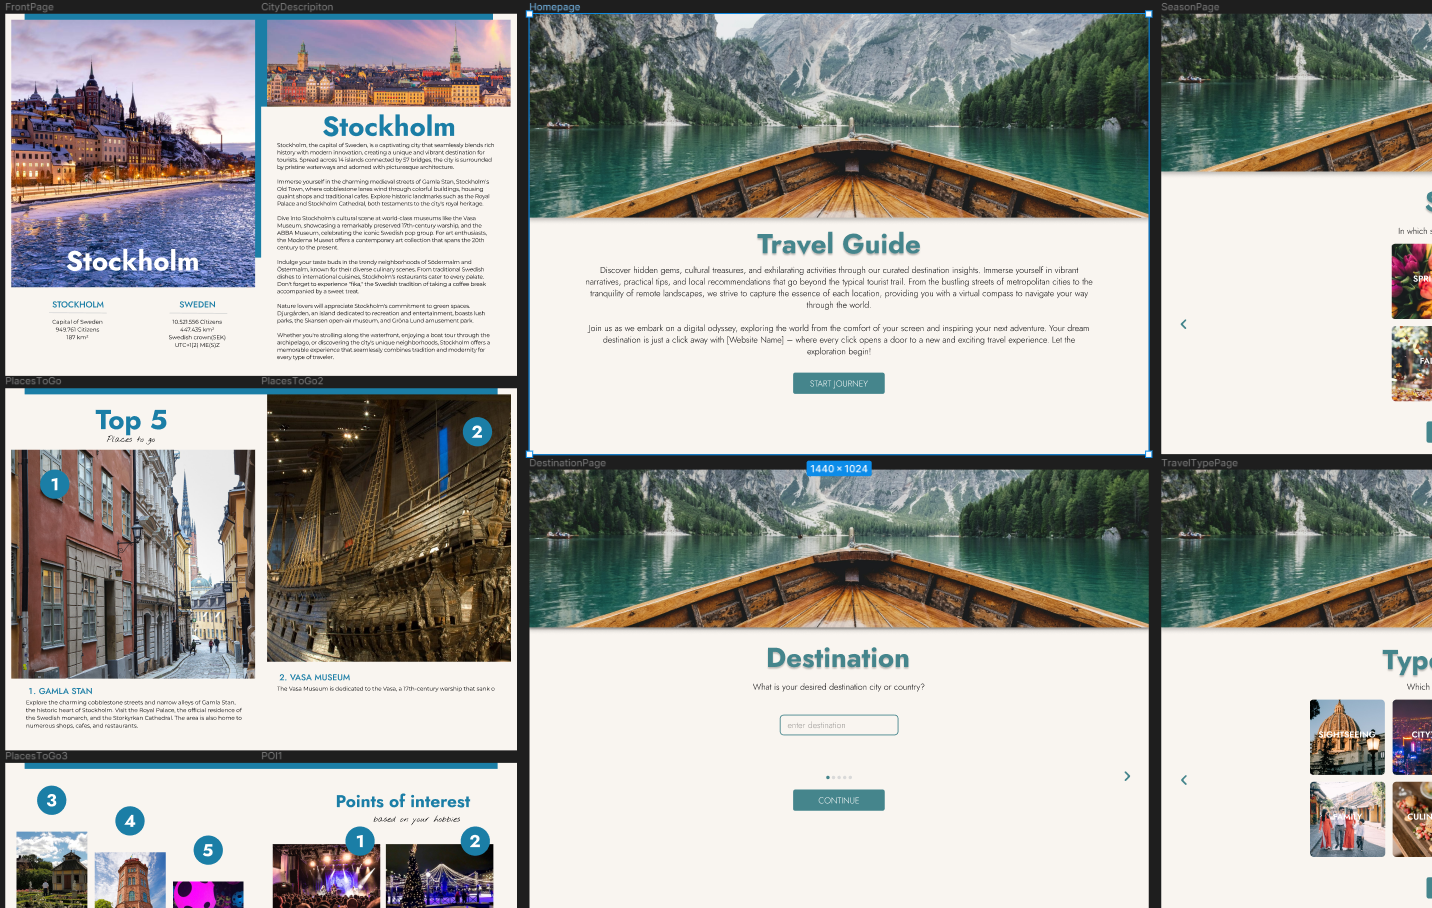
\includegraphics[width=1\textwidth]{Mockup_Example.png}
	\caption{Mockup of Applicaton and Guide}
	\label{fig1}
\end{figure}

Equipped with insights gleaned from our survey, we embarked on the development of an initial mockup for Guide Guru. Leveraging Figma\footnote{https://www.figma.com/de}, a collaborative design tool, we crafted a clickable prototype encompassing the entire user journey and a blueprint for our PDF guide. This mockup (see figure  \ref{fig1}) enabled us to pinpoint necessary input parameters, map out pages, identify reusable components, and discover the inherent structure of our web application in a fast and efficient manner.


\section{Implementation First Prototype}
 

\section{User Testing}

Conducting user testing with potential users is a crucial step in ensuring the quality of a prototype and identifying any potential bugs or errors that developers may overlook. By involving 5 potential users in testing our first iteration of the prototype, we aimed to gain qualitative insights into possible user journeys and identify any usability issues or challenges they encountered.

\subsection{Findings}

At the start of the test, each user received a brief introduction about what the test would cover. They were asked to imagine themselves planning a specific journey and to enunciate their thoughts on the interaction. After this initial introduction, users were not given any further instructions on how to use the prototype.

Some key findings from our user tests were that users expressed a desire to search not just for cities, but also for countries in order to select a city located within a specific country. Additionally, users noted that listing the country alongside city options could prevent errors in selection, especially when cities share the same name. The text displayed on input cards was considered insufficiently legible. On the result page, which included a sample guide, it led to confusion among users when the guide featured a different city from the one they had selected.

One user encountered a bug that disabled the large language model. This occurred when the user attempted to use the \texttt{select all} option within the selection of additional hobbies, resulting in the prompt exceeding its maximum length and causing the backend to shut down. Another user selected a hobby that was unavailable in the destination city, prompting the language model to generate an apology stating it couldn't find relevant data, which was then displayed in the guide.


\subsection{Further Enhancements}
Two of the five test user would like to include an duration of the vacation an thus an suitable amount of places of interest for that duration. Three users thought of ideas to avoid the generation time with facts or images about the destination or an pageful output of the guide. Only one thought that the travel guide contained incorrect information for the places of interest. The user thought that probably two niche hobbies would not be part of an tournament in the same park.

Two out of the five test users expressed interest in including the duration of the vacation to determine a suitable number of places of interest for that period. Three users brainstormed ideas to mitigate generation time, such as incorporating facts or images about the destination or showing the result of each fully generated page as soon as it was available. Only one user thought that the travel guide provided incorrect information regarding the places of interest. The guide stated that two niche hobbies have independent tournaments in the same park. Further research didn't provide any information about the tournaments in this park so the description of the place was presumably wrong.

\section{Final Prototype}

\section{Challenges}


\section{Lessions Learned}



%%%-----------------------------------------------------------------------------
\chapter{System Documentation}
%%%-----------------------------------------------------------------------------

%Give a well-structured description of the architecture and the technical design
%of your implementation with sufficient granularity to enable an external person
%to continue working on the project.

\section{Backend}
%Example for code documentation
%CSSCode, HtmlCode or JsCode
\begin{PythonCode}
	import numpy as np
	
	def incmatrix(genl1,genl2):
	m = len(genl1)
	n = len(genl2)
	M = None #to become the incidence matrix
	VT = np.zeros((n*m,1), int)  #dummy variable	
\end{PythonCode}

\subsection{Backend API with Flask}
In this section, we will establish the backend API using Flask. Flask is a prominent Python web framework utilized for building RESTful APIs. We chose this framework because of its simplicity and flexibility. Our goal was to create a backend infrastructure that integrates Flask and ChatGPT functionalities. The API enables communication between the user interface and the AI model, ensuring efficient query handling and response generation. The Flask API looks like the following:
\begin{PythonCode}
	class ChatHandler(Resource):
	def __init__(self, **kwargs):
	self.context = [{"role": "system", "content": system_context}]
	
	def get(self):
	response = jsonify(context=self.context)
	response.headers.add("Access-Control-Allow-Origin", "*")
	return response
	
	def post(self):
	rqs = request.json
	print(f'POST Print RQS: {rqs}\n')
	destination = rqs.get('destination')
	seasons = rqs.get('seasons')
	travelType = rqs.get('travelType')
	hobbies = rqs.get('hobbies')
	addHobbies = rqs.get('addHobbies')
	country = rqs.get('country')
	
	print(f'POST: {destination}\n{country}\n')
	
	response = jsonify(get_response(destination, hobbies, travelType, seasons, addHobbies, country))
	return response
	
	
	api.add_resource(ChatHandler, '/')
\end{PythonCode}
The API handles HTTP POST requests which are made to the endpoint '/'. The post method retrievs the sent JSON and extracts relevant information such as destination, seasons, travel type, hobbies, additional hobbies, and country. The extracted data is then passed to the function get\_response() from the utility module which processes these user's preferences and will generate a suitable response with information about the destination and personalized recommendations


\subsection{Large Language Model Integration}

\subsection{Integration of Google APIs}

\subsection{Geonames API} \label{GeonamesAPI}
We utilized the geonames API to validate user input while keeping the range of possible destinations open. The geonames API contains data on approximately 4.8 million populated places, including details such as name, alternative names, country, population, geolocation, and categorization. To refine the user options, we set a threshold of including only places with over 1,000 inhabitants, ensuring that the travel guide's output remains relevant and accurate.

For the integration of this API into our Guide Guru, we used Express.js\footnote{https://expressjs.com/de/} to create the API Interface. After incorporating cors and axios middleware, we developed two interfaces for communicating with the geonames API.

To enhance user experience, we designed a mechanism to display only well-known and populous destinations upon the initial opening of the dropdown field. Upon rendering the destination page, a request is triggered, prompting an axios-request to the geonames API which can be seen in the below code. This request retrieves 25 cities with over 15,000 residents in its response, ensuring that users are presented with familiar and prominent locations.

\begin{JsCode}
app.get('/api/bigCity', (req, res) => {
	const apiUrl = 'http://api.geonames.org/searchJSON?cities=cities15000&maxRows=25&username=fhtravelguidews23';
	axios.get(apiUrl)
	.then(response => {
		res.json(response.data)
	})
	.catch(error => {
		console.error('Error fetching data:', error);
	});
});
\end{JsCode}

As soon as the user begins to enter into the input field an request is sended for ten places that match the input an have more than 1,000 citicens to allow a high variety of possible travel destinations. 

Once the user starts typing in the input field, a request is sent to retrieve ten places that match the input criteria and have more than 1,000 inhabitants, thus providing a diverse range of potential travel destinations.

The processing of the API response data is detailed in the description of our Destination Page at \ref{DestinationPage}.

\section{Frontend}

As mentioned previously, we opted for React as our frontend technology. To maintain a component-based architecture, we divided our frontend into pages that leverage multiple components we designed and implemented. Additionally, we established a state management system to store both user input and data provided by the backend. This mixture of technologies enables us to create a straightforward yet efficient user journey.

\subsection{State Management}
For state management, we utilized the Redux library to store both user input and data retrieved from the backend. The  \texttt{inputSlice.js} file is responsible for storing the input of the user regarding the desired destination, seasons, type of travel, and selected hobbies they want to include in their journey. Additionally, we implemented a function within this slice to reset the user's input for new requests without requiring a page reload.

Within the \texttt{guideSlice.js} file, all information necessary to construct the guide is saved. This includes details such as destination, population, area, longitude, latitude, country information, images with appropriate dimensions, and recommended places.

In the file \texttt{store.ts}, these two reducers are configured and made accessible within the store variable. For instance, \texttt{store.getState().userInput.destination} provides access to the user's selected destination. To add data into the store, you can use functions like  \texttt{dispatch(setDestionation("destination"))}.

\subsection{Pages}

In our mockup design, we implemented separate pages for each stage of the user journey. Each page features the header component, providing a consistent element throughout the experience for user familiarity. To ensure the validity of every guide request, we opted against traditional navigation methods and instead enabled users to navigate solely using buttons located at the bottom of each page.

\subsubsection{Homepage}

The homepage serves as the initial step in the user journey. To facilitate a seamless start to their personalized experience, we included our logo and a brief introduction explaining how to use the application. Additionally, to encourage continued engagement with the website, we incorporated a call to action featuring a button labeled \textit{Start your journey}, directing users to the first input page.

\begin{figure}
	\centering
	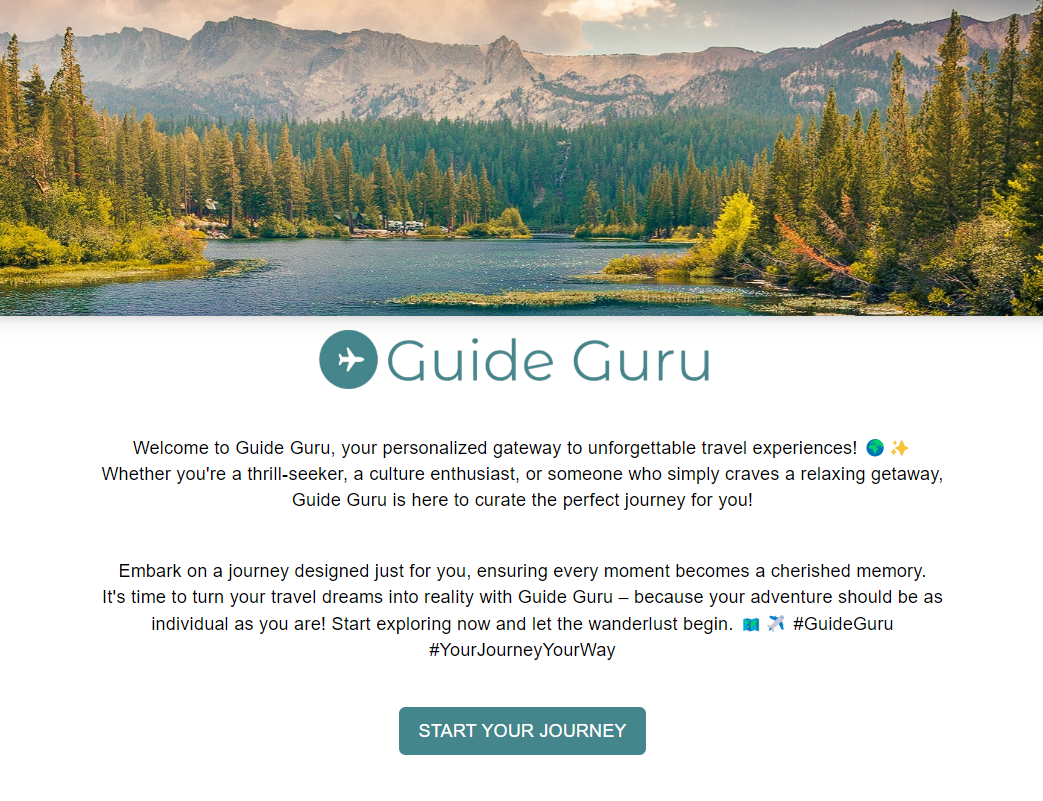
\includegraphics[width=1\textwidth]{Homepage.png}
	\caption{Homepage of Guide Guru}
\end{figure}

\subsubsection{Destination}\label{DestinationPage}

In the destination page, users are prompted to choose their preferred travel destination from options provided by our geonames API interface. Upon the initial rendering of the page, a request is made for 25 cities with more than 15,000 inhabitants. The responses from this interface populate the options, where the city name serves as the value and part of the label, along with the country name to prevent confusion between places with similar names. Additionally, information such as city population, country, latitude, and longitude is included in the options to be stored in the state when the user selects a destination. We utilized the \texttt{react-select} library to build this selection component, and the required HTML structure is as follows:

\begin{HtmlCode}
	<form onSubmit={formSubmit}>
		<div className="my-4 flex justify-center">
			<Select
				isSearchable={true}
				options={cityOptions}
				onInputChange={loadOptions}
				required={true}
				onChange={handleChange}
				placeholder="start typing or select a city ..."
			/>
		</div>
		<Button text='Continue' type='submit'/>
	</form>
\end{HtmlCode}

To send requests to the interface and build the adapted options as described above when the user starts typing into the input field, we utilize the following TypeScript function. This function is called from the \texttt{onInputChange} event of the \texttt{<Select>} component:

%CSSCode, HtmlCode or JsCode
\begin{JsCode}
const [cityData, setCityData] = useState([]);
const [cityOptions, setCityOptions] = useState([]);
const dispatch = useDispatch();
	
const loadOptions = (inputValue: string) => {
	axios.get('http://127.0.0.1:4000/api/city?city=' + inputValue, {}).then((response) => {
		setCityData(response.data.geonames);
	}).catch(error => console.log(error));
};

useEffect(() => {
	createOptions();
}, [cityData]);

function createOptions() {
	const newOptions = []
	cityData.forEach((city) => {
		newOptions.push({
			...city.name,
			value: city.name,
			label: city.name + ' (' + city.countryName + ')',
			population : city.population,
			country: city.countryName,
			lat: city.lat,
			lng: city.lng,
		})
	})
	setCityOptions(newOptions);
}

const handleChange = (selectedOption) => {
	dispatch(setDestination(selectedOption.value));
	let cityCiticens = selectedOption.population.toString().replace(/\B(?=(\d{3})+(?!\d))/g, ",");
	dispatch(setCitizens(cityCiticens));
	dispatch(setCountry(selectedOption.country));
	dispatch(setLatitude(selectedOption.lat));
	dispatch(setLongitude(selectedOption.lng));
};
\end{JsCode}

Within the \texttt{loadOptions} function, a request is made to the interface, and the hook for \texttt{cityData} is adapted accordingly. This change triggers the \texttt{useEffect}, which constructs the new options for the selection, refreshing the \texttt{cityOptions} hook.

Once the user selects a destination, the \texttt{handleChange} function is accessed. This function adds the necessary and formatted information into the stores. Therefore, the required data is already saved, and the \texttt{onSubmit} function simply redirects to the next page.

\subsubsection{Seasons}

On the season page, users are required to select at least one of the four seasons. The selection methodology is described within the \texttt{CardBlock} component at \ref{CardBlockComponent}. To ensure that the user has selected at least one season, the form submission process checks the season store for elements. If the season store is empty, the message indicating the selection requirements switches from the regular color to bold red as can be seen in the HTML and TypeScript code below.

\begin{HtmlCode}
<form onSubmit={handleSubmit(onSubmit)}>
	<Heading headingLevel='h3' text="In which season would you like to travel?"/>
	<Paragraph text="Select one or multiple seasons for your journey." 
		className={`${textColor} ${isBold ? 'font-bold' : ''}`}/>
	<CardBlock category="seasons" name="seasons"/>
</form>
\end{HtmlCode}


\begin{JsCode}
const navigate = useNavigate();
const [textColor, setTextColor] = useState('text-black');
const [isBold, setIsBold] = useState(false);

function formSubmit(data: UserInput) {
	if (store.getState().userInput.seasons.length === 0) {
		setTextColor('text-error');
		setIsBold(true);
	} else {
		navigate('/type');
	}
}

const onSubmit: SubmitHandler<UserInput> = data => formSubmit(data);	
\end{JsCode}


Once the requirements are met, the user is redirected to the travel type page.

\subsubsection{Travel Type}

The functionality of the travel type page mirrors that of the seasons page. Users must select at least one element in the \texttt{CardBlock} component to ensure a correct output from the large language model. Additionally, this requirement aims to motivate users to enter a category, which will be used to tailor the guide to their individual needs.

\begin{figure}
	\centering
	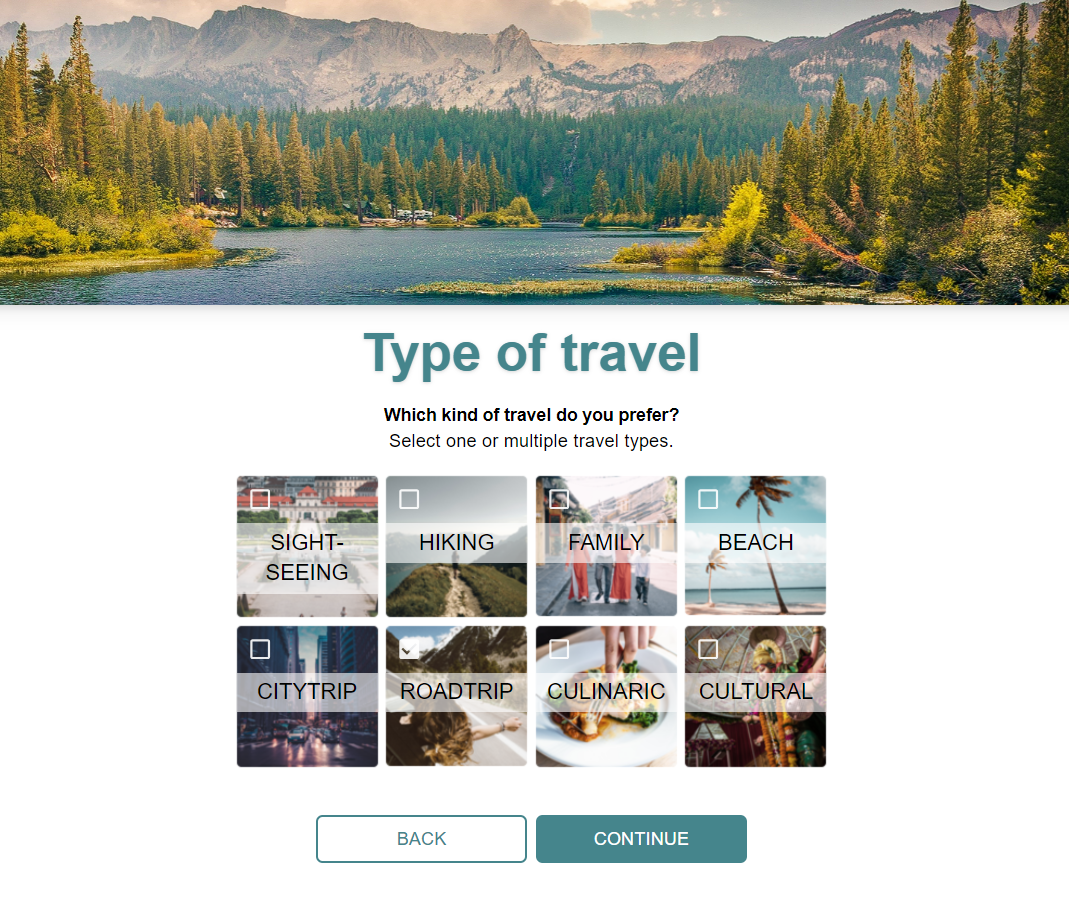
\includegraphics[width=1\textwidth]{TravelType.png}
	\caption{Selection of the type of travel}
\end{figure}


\subsubsection{Hobbies}
The hobby page shares similarities with the previous pages, but includes three different \texttt{CardBlock} components, one of which contains the \texttt{HobbySelection} component described at \ref{HobbySelectionComponent}. 

To ensure tailored and appropriate travel guide outputs, we've increased the minimum selected options to three hobbies, either inside the \texttt{CardBlock} or the \texttt{HobbySelection} component. This adjustment aims to prevent undefined or incorrect outputs for points of interest when selected hobbies are not possible at the chosen destination (\eg, skiing in Hawaii). By requiring at least three hobbies to be selected, we anticipate that the guide will provide some relevant points of interest.

The functionality of this page remains largely the same, but includes a small computation for the \texttt{CardBlock} and the additional selected hobbies in the \texttt{HobbySelection} component, as demonstrated below.

\begin{JsCode}
	const [textColor, setTextColor] = useState('text-black'); 
	const [isBold, setIsBold] = useState(false);
	
	function formSubmit(data: UserInput) {
		const totalHobbies = store.getState().userInput.hobbies.length + 
			store.getState().userInput.addHobbies.length;
		if (totalHobbies < 3) {
			setTextColor('text-error');
			setIsBold(true);
		} else {
			navigate('/result');
		}
	}	
\end{JsCode}

\subsubsection{Result}


At the result page, users are presented with their personal input. We've provided users with the option to validate their input before generating the guide. This is important because the guide generation process can take one to two minutes of computation time, and users should have the possibility to establish it when they are pleased with their input. On this page, users can navigate to each of the previous input pages and change their selection or start a new travel guide with new parameters.

When the user clicks on the generate button, a request with the stored input data is sent to the backend to be computed by the large language model. The resulting guide is then stored in the \texttt{guideStore} to be accessed in the generated PDF document (see \ref{ReactPDF}), to which the user is subsequently redirected.

In the code below the request to the backend to generate the guide and the handling of the output is shown:

\begin{JsCode}
	const fetchChatResponse = () => {
		setIsLoading(true); // shows the loading animation, interactive map and message
		
		// load the stored inputs
		const destination = store.getState().userInput.destination;
		const seasons = store.getState().userInput.seasons;
		const travelType = store.getState().userInput.travelType;
		const hobbies = store.getState().userInput.hobbies;
		const addHobbies = store.getState().userInput.addHobbies;
		const country = store.getState().guide.country.name;
		
		// request to the LLM
		axios.post('http://127.0.0.1:5000/', {
			destination: destination,
			seasons: seasons,
			travelType: travelType,
			hobbies: hobbies,
			addHobbies: addHobbies,
			country: country
		}).then((response) => {
			// save data into guideStore
			dispatch(setDescription(response?.data.destination_text));
			dispatch(setDestination(destination));
			dispatch(setArea(shortenAnswerForNumbers(response?.data.city_area)));
			dispatch(setCountryCitizens(shortenAnswerForNumbers(response?.
				data.country_citicens)));
			dispatch(setCountryArea(shortenAnswerForNumbers(response?.
				data.country_area)));
			dispatch(setCurrency(response?.data.currency));
			let places = response?.data.places_text;
			let placesArr = places.split(/: |\n\n/);
			dispatch(setPlacesToGo(placesArr))
			places = response?.data.poi_text;
			placesArr = places.split(/: |\n\n/);
			dispatch(setPOI(placesArr));
			setIsLoading(false);
			navigate('/exportGuide')
		}).catch(error => console.log(error));
	};
\end{JsCode}

During the guide generation process, the user is notified that it may take some time. Additionally, an interactive map component (see \ref{InteractiveMap}) is displayed, showing the selected destination marked with data retrieved from the geonames API (described at \ref{GeonamesAPI}). This allows the user to explore their chosen travel destination while waiting for the guide to be generated.

\begin{figure}
	\centering
	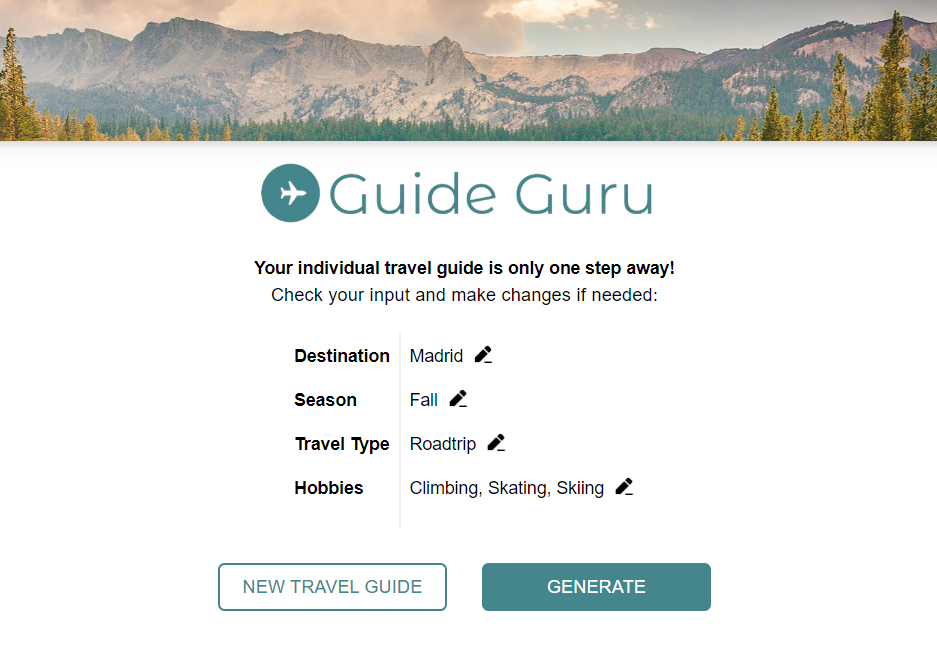
\includegraphics[width=0.4\textwidth]{ResultPage.png}
	\caption{Result page before generation}
	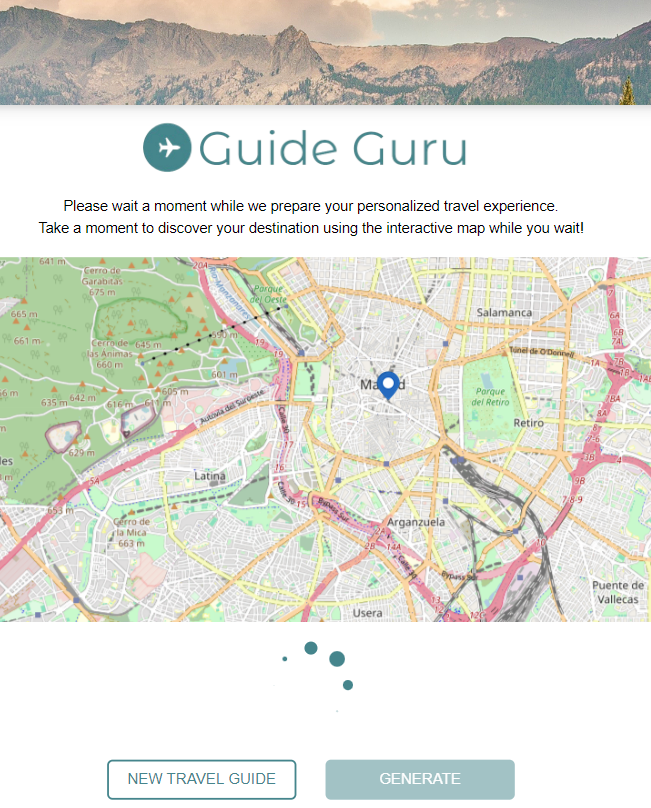
\includegraphics[width=0.4\textwidth]{ResultPageLoading.png}
	\caption{Result page during generation}
\end{figure}

\subsubsection{Export Guide}

This page is only needed to include the PDF Viewer and the React PDF that is described in the subsection \ref{ReactPDF}. 

\subsection{Components}

\subsubsection{Button}

\subsubsection{CardBlock} \label{CardBlockComponent}

\subsubsection{CardInput}

\subsubsection{Header}

\subsubsection{Heading}

\subsubsection{HobbySelection} \label{HobbySelectionComponent}

\subsubsection{InteractiveMap} \label{InteractiveMap}

\subsubsection{Paragraph}

\subsection{React-PDF} \label{ReactPDF}

React-PDF renderer is a library utilized for generating PDF files with a markup structure similar to HTML and CSS. This enables easy integration into any application. To enable the browser to open the generated PDF, a \texttt{<PDFViewer>} element is required, within which a \texttt{<Document>} is created. Then, as many \texttt{<Pages>} as necessary can be added to the document. To structure the layout of the PDF, the \texttt{<View>} element can be utilized. For including text and images, the appropriate \texttt{<Text>} and \texttt{<Image src="path/to/image">} elements can be used. With these components, we were able to create the simple yet effective layout of our travel guide, as depicted in \ref{fig2}.

\begin{figure}
	\centering
	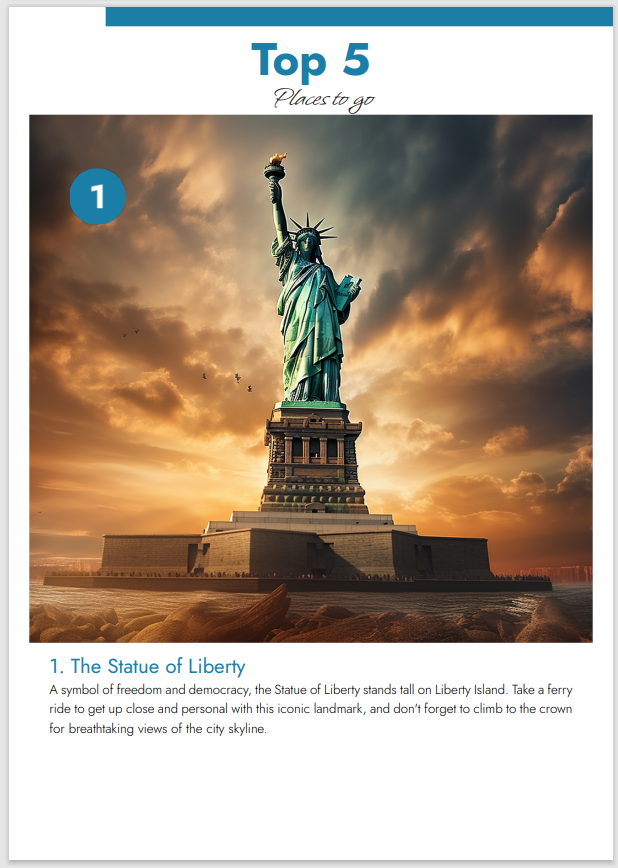
\includegraphics[width=0.4\textwidth]{Guide_NY_Top5.png}
	\caption{Front page of the travel guide}
	\label{fig2}
	
	\begin{HtmlCode}
<PDFViewer style={styles.viewer}>
	<Document>
		<Page size="A4" style={styles.page}>
			<div style={styles.pageAccent}></div>
				<View style={styles.section}>
					<Text style={styles.title}>Top 5</Text>
					<Text style={styles.handwritten}>Places to go</Text>
					<Image src="../src/img/pdf/imgs/image_3.jpg" 
						style={styles.largeImg}></Image>
					<Image src="../src/img/pdf/icons/Icon1.png" style={[styles.numIcon, 
						{ position: 'absolute', top: 150, left:50}]}></Image>
					<View style={styles.section}>
					<Text style={styles.headingLg}>{placesToGo.first.name}</Text>
					<Text style={styles.description}>{placesToGo.first.description}</Text>
				</View>
			</View>
		</Page>
 </Document>
</PDFViewer>
	\end{HtmlCode}
\end{figure}
For styling the PDF, it is possible to utilize the \texttt{style} attribute on every component of the React-PDF library. To enhance code readability and separation of concerns, we decided to store our styling in a separate variable. In the code snipped below the definition of the style elements used in the code in \ref{fig3} can be seen:
\begin{figure}
\begin{CssCode}
const styles = StyleSheet.create({
	viewer: {
		width: window.innerWidth, 
		height: window.innerHeight,
	},
	page: {
		backgroundColor: 'rgba(255,255,255,0.6)',
		color: "white",
		fontFamily: 'Jost',
	},
	pageAccent: {
		width: 500,
		height: 20,
		position: "absolute",
		right: 0,
		backgroundColor: '#1B7EA6'
	},
	title: {
		color: '#1B7EA6',
		fontSize: 45,
		textAlign: 'center',
		fontFamily: 'Jost',
		fontWeight: "bold"
	},
	section: {
		margin: 10,
		padding: 10,
		color: 'black',
	},
	headingLg: {
		width: ImageDimensions.large.width,
		fontSize: 20,
		color: '#1B7EA6',
	},
	handwritten: {
		fontFamily: 'Handwritten',
		textAlign: "center",
		color: '#232323',
		fontSize: 28,
		position: "absolute",
		top: 63,
		left: 250,
	},
	largeImg:{
		top: 22,
		height: ImageDimensions.large.height,
		marginBottom: 10,
		objectFit: "cover",
	},
	numIcon:{
		height: ImageDimensions.icon.height,
		width: ImageDimensions.icon.width,
		alignSelf:"center",
		marginBottom: 30,
	},
	description:{
		fontSize: 13,
		fontWeight: "light",
	}
});
\end{CssCode}
\caption{Styling of page depicted at \ref{fig2}}
\label{fig3}
\end{figure}
%%%-----------------------------------------------------------------------------
\chapter{Summary}
%%%-----------------------------------------------------------------------------

Give a concise (and honest) summary of what has been accomplished and what not. 
Point out issues that may warrant further investigation.

%%%-----------------------------------------------------------------------------
\appendix                                                   % Switch to appendix
%%%-----------------------------------------------------------------------------

%%%-----------------------------------------------------------------------------
\chapter{Supplementary Materials}
%%%-----------------------------------------------------------------------------

The appendix is a good place to attach a user guide, screenshots, installation
instructions, etc. Add a separate chapter for each major item.

%%%-----------------------------------------------------------------------------
\MakeBibliography[nosplit]
%%%-----------------------------------------------------------------------------

%%%-----------------------------------------------------------------------------
\end{document}
%%%-----------------------------------------------------------------------------
